\documentclass[dvipdfmx,11pt,notheorems]{beamer}
%%%% 和文用 %%%%%
\usepackage{bxdpx-beamer}
\usepackage{pxjahyper}
\usepackage{minijs}%和文用
\usepackage{listings,jlisting} % プログラムの表示用
\renewcommand{\kanjifamilydefault}{\gtdefault}%和文用

%%%% tikz 用 %%%%%
\usepackage[latin1]{inputenc}
\usepackage{tikz}
\usetikzlibrary{intersections}
\usetikzlibrary{shapes,arrows}

%%%% スライドの見た目 %%%%%
\usetheme{Boadilla}
\usecolortheme{seahorse}
\usefonttheme{professionalfonts}
\setbeamertemplate{frametitle}[default][center]
\setbeamertemplate{navigation symbols}{}
\setbeamercovered{transparent}%好みに応じてどうぞ)
\setbeamertemplate{footline}[page number]
\setbeamerfont{footline}{size=\normalsize,series=\bfseries}
\setbeamercolor{footline}{fg=black,bg=black}

\setbeamercolor{white-cyan1}
{fg=white,bg=cyan!80!black}
\setbeamercolor{white-cyan2}
{fg=white,bg=cyan!60!black}
%%%%

%%%% 定義環境 %%%%%
\usepackage{amsmath,amssymb}
\usepackage{amsthm}
\theoremstyle{definition}
\newtheorem{theorem}{定理}
\newtheorem{definition}{定義}
\newtheorem{proposition}{命題}
\newtheorem{lemma}{補題}
\newtheorem{corollary}{系}
\newtheorem{conjecture}{予想}
\newtheorem*{remark}{Remark}
\renewcommand{\proofname}{}
%%%%%%%%%

%%%%% フォント基本設定 %%%%%
% \usepackage[T1]{fontenc}%8bit フォント
% \usepackage{textcomp}%欧文フォントの追加
% \usepackage[utf8]{inputenc}%文字コードをUTF-8
% \usepackage{otf}%otfパッケージ
% \usepackage{lxfonts}%数式・英文ローマン体を Lxfont にする
% \usepackage{bm}%数式太字
%%%%%%%%%%

%%%%% 複数人の著者を揃える %%%%%
%% http://tex.stackexchange.com/questions/
%%   166531/how-to-change-author-alignment-in-beamer
\makeatletter
\long\def\beamer@author[#1]#2{%
  \def\insertauthor{\def\inst{\beamer@insttitle}\def\and{\beamer@andtitle}%
  \begin{tabular}{rl}#2\end{tabular}}%
  \def\beamer@shortauthor{#1}%
  \ifbeamer@autopdfinfo%
    \def\beamer@andstripped{}%
    \beamer@stripands#1 \and\relax
    {\let\inst=\@gobble\let\thanks=\@gobble\def\and{, }\hypersetup{pdfauthor={\beamer@andstripped}}}
  \fi%
}
\makeatother
%%%%%%%%%%

%%%%% プログラムに色をつける
\usepackage{color}

\definecolor{codegreen}{rgb}{0,0.6,0}
\definecolor{codegray}{rgb}{0.5,0.5,0.5}
\definecolor{codepurple}{rgb}{0.58,0,0.82}
\definecolor{backcolour}{rgb}{0.95,0.95,0.92}

\lstdefinestyle{mystyle}{
    backgroundcolor=\color{backcolour},
    commentstyle=\color{codegreen},
    keywordstyle=\color{magenta},
    numberstyle=\tiny\color{codegray},
    stringstyle=\color{codepurple},
    basicstyle=\footnotesize,
    breakatwhitespace=false,
    breaklines=true,
    captionpos=b,
    keepspaces=true,
    numbers=left,
    numbersep=5pt,
    showspaces=false,
    showstringspaces=false,
    showtabs=false,
    tabsize=2
}

\lstset{style=mystyle}

%%%%
\title[略タイトル]{第2回 知能システム学特論レポート}%[略タイトル]{タイトル}
\author[NishidaLab]{
15344203 & 有田 裕太 \\
15344206 & 緒形 裕太 \\
15344209 & 株丹 亮 \\
12104125 & 宮本 和 }%[略名前]{名前}
\institute[NishidaLab]{西田研究室,計算力学研究室}%[略所属]{所属}
\date{2015年\ 6月\ 25日}%日付

\begin{document}

%%%% 1 %%%%
\begin{frame}[plain]\frametitle{}
\titlepage %表紙
\end{frame}

% \begin{frame}\frametitle{Contents}
% \tableofcontents %目次
% \end{frame}

\section{進捗状況}
%%%% 2 %%%%
\begin{frame}\frametitle{進捗状況}

\begin{block}{理論研究の進捗}
人工ニューラルネットワーク・caffeについて調べた
\end{block}

\vspace{1cm}
\begin{exampleblock}{プログラミングの進捗}
中間層の出力,可視化を模索中
\end{exampleblock}
\end{frame}

%%%% 3 %%%%

\begin{frame}[fragile]\frametitle{人工ニューラルネットワーク}
\begin{block}{誤差逆伝搬法}
80年から90年代,誤差逆伝搬法(back propagation)が多層ニューラルネットワークの学習方法として確立
\end{block}

しかし,誤差逆伝搬法で学習可能なのは2層程度\\

\begin{block}{問題点}
多い層をもつニューラルネットワークの学習では様々な問題により上手く学習することが出来ない
\end{block}
\begin{itemize}
\item 単相ネットワークに分解し,入力層に近い側から順番に教師なしで学習する
\item 目的とするニューラルネットワークの学習前に層ごとに学習を行うことで良い初期値パラメータを求めておくやり方を事前学習(pretraining)という
\end{itemize}
\end{frame}

%%%% 4 %%%%
\begin{frame}[fragile]\frametitle{caffe}
 caffe - CNN(Convolutional Neural Networks)の実装
\vspace{0.2cm}

\hfill
\begin{beamercolorbox}[ center, wd=60mm, sep=2pt, shadow=false, rounded=true ]{white-cyan1}
 イメージを入力
\end{beamercolorbox}
\hfill\hfill

\vspace{0.2cm}

\hfill
\begin{beamercolorbox}[ center, wd=60mm, sep=2pt, shadow=false, rounded=true ]{white-cyan2}
低次元の特徴検出 (単純な形状など)
\end{beamercolorbox}
\hfill\hfill

\vspace{0.2cm}

\hfill
\begin{beamercolorbox}[ center, wd=60mm, sep=2pt, shadow=false, rounded=true ]{white-cyan1}
高次元の特徴検出 (複雑な形状)
\end{beamercolorbox}
\hfill\hfill

\vspace{0.2cm}

\hfill
\begin{beamercolorbox}[ center, wd=60mm, sep=2pt, shadow=false, rounded=true ]{white-cyan2}
画像全体を把握
\end{beamercolorbox}
\hfill\hfill

\vspace{0.2cm}

\hfill
\begin{beamercolorbox}[ center, wd=80mm, sep=2pt, shadow=false, rounded=true ]{white-cyan1}
オブジェクトを形成する不変の要素を把握
\end{beamercolorbox}
\hfill\hfill

\vspace{0.2cm}

学習により自動でオブジェクトを区分できるようになる
\end{frame}

%%%% 5 %%%%
\begin{frame}\frametitle{今後の課題}

\begin{block}{理論研究}
DNN,CNN,caffeについて理解を深める
\end{block}

\vspace{1cm}
\begin{exampleblock}{プログラミング}
中間層の出力,可視化
\end{exampleblock}
\end{frame}

% \begin{figure}[t]
%  \begin{minipage}{0.3\hsize}
%   \centering
%   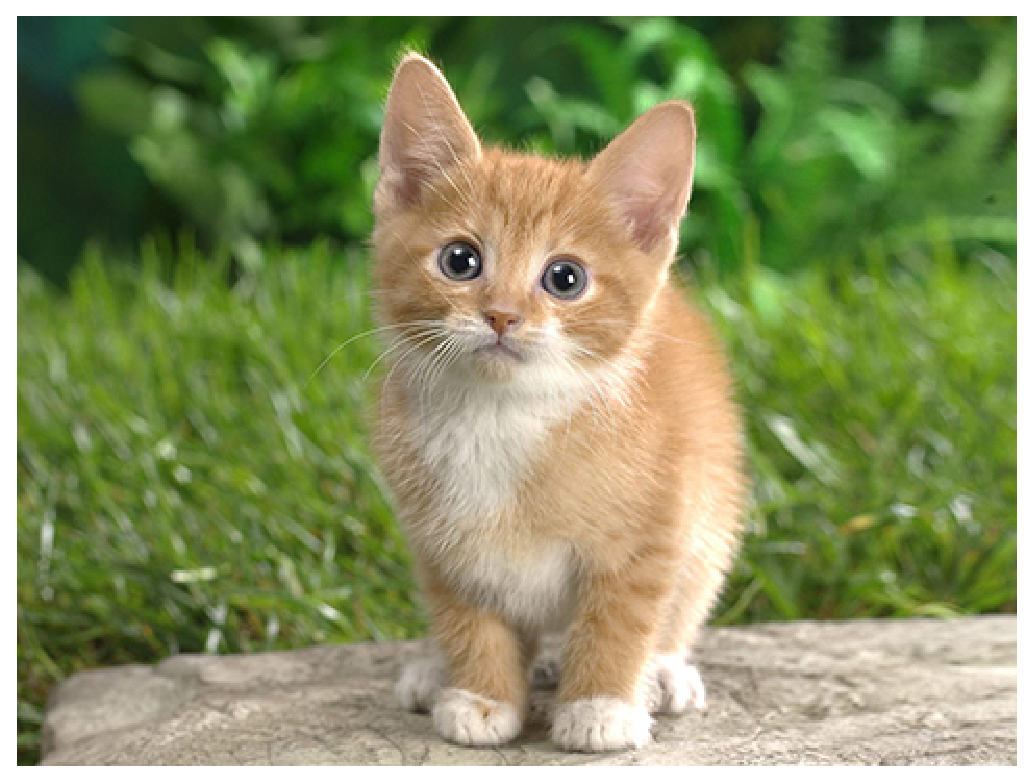
\includegraphics[width=30mm]{./figure/cat.eps}
%   \caption{cat.jpg}
%   \label{sample1}
%  \end{minipage}
%  \begin{minipage}{0.3\hsize}
%   \centering
%   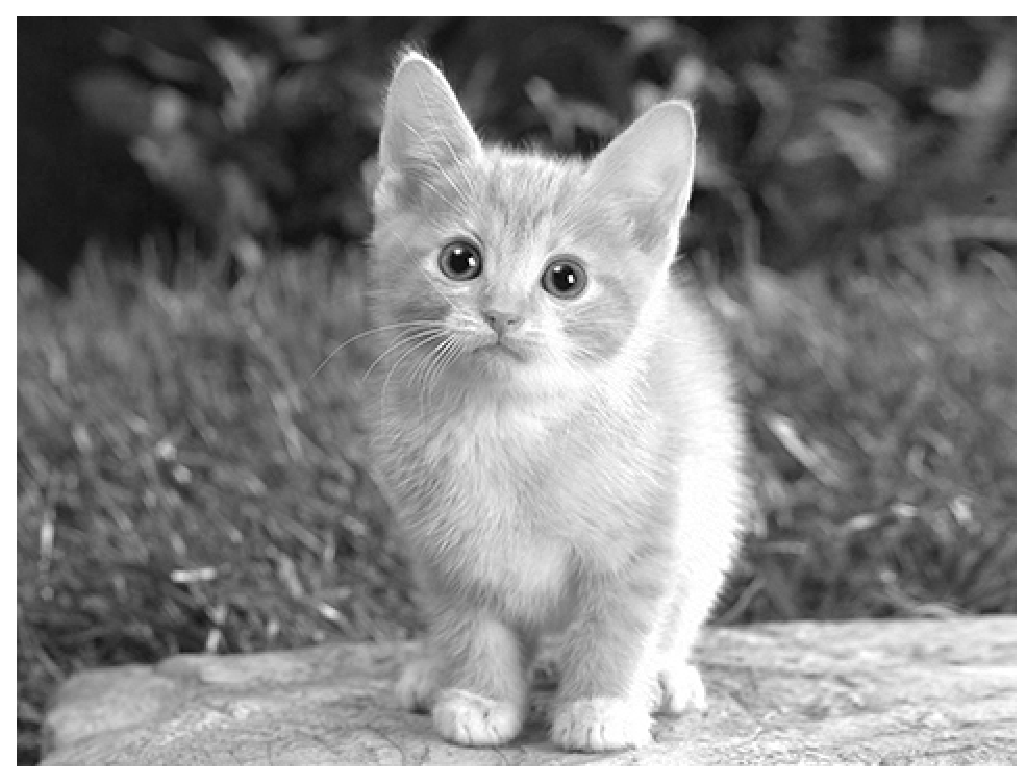
\includegraphics[width=30mm]{./figure/cat_gray.eps}
%   \caption{cat\_gray.jpg}
%   \label{sample2}
%  \end{minipage}
%  \begin{minipage}{0.3\hsize}
%   \centering
%   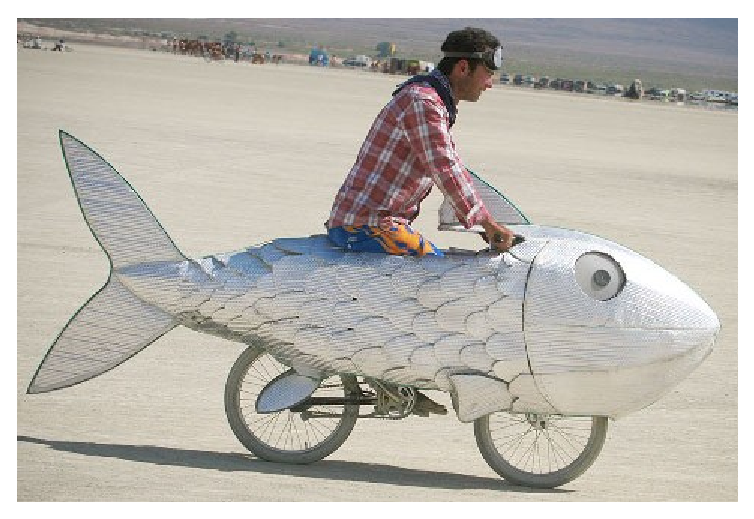
\includegraphics[width=30mm]{./figure/fish-bike.eps}
%   \caption{fish-bike.jpg}
%   \label{sample3}
%  \end{minipage}
% \end{figure}
% \begin{exampleblock}{実行環境}
% \begin{itemize}
%  \item Ubuntu 14.04 LTS
%  \item Intel core i5-4440 3.10GHz$\times$4
%  \item RAM 16GB
% \end{itemize}
% \end{exampleblock}
% \end{frame}


% \section{具体例}

% \begin{frame}\frametitle{定理環境の例}
% \begin{theorem}[Fermat]
% $a^{p-1} \equiv 1 \pmod{p}$
% \end{theorem}
% \pause
% \begin{theorem}[Wilson]
% \begin{equation}
% (p-1)! \equiv 1 \pmod{p}
% \end{equation}
% \end{theorem}
% \end{frame}

% \begin{frame}<1-2>\frametitle{オーバーレイ}
% \onslide*<1>{
% \Large{これは1枚目です}
% }
% \onslide*<2>{
% これは2枚目です
% \begin{theorem}[Euclid]
% There is no largest prime number.
% \end{theorem}
% }
% \end{frame}

% \begin{frame}\frametitle{色もつけれるよ}
%   {\color{red} red}(\alert{alert}),
%   {\color{blue} blue}(\structure{structure}),
%   {\color{green} green},
%   {\color{cyan} cyan},
%   {\color{magenta} magenta},
%   {\color{yellow} yellow},
%   {\color{black} black},
%   {\color{darkgray} darkgray},
%   {\color{gray} gray},
%   {\color{lightgray} lightgray},
%   {\color{orange} orange},
%   {\color{violet} violet},
%   {\color{purple} purple},
%   {\color{brown} brown},
% \end{frame}

% \begin{frame}\frametitle{いろんなブロック}
% \begin{block}{ブロック}
% これは普通のブロックです
% \end{block}

% \begin{alertblock}{警告ブロック}
% 警告!これは警告ブロックだ!
% \end{alertblock}

% \begin{exampleblock}{例ブロック}
% 例えば、こんなブロックです。
% \end{exampleblock}
% \end{frame}

% \begin{frame}<1-2>\frametitle{画像も貼れるよ}
% \onslide*<1>{
% このように画像を貼れるよ
% %\begin{figure}[htb]
% %\centering
% %\includegraphics[width=12cm,clip]{dummygraph.pdf}
% %\caption{$f(x)=e^{-\frac{x}{10}}\sin(x)$}
% %\end{figure}%
% }
% \onslide*<2>{
% 画像や表は各自用意してね
% %\begin{figure}[htb]
% %\centering
% %\includegraphics[width=8cm,clip]{sym4.pdf}
% %\caption{Cayley graph of $\mathfrak{S}_{4}$}
% %\end{figure}%
% }
% \end{frame}

% \begin{frame}\frametitle{まとめ}
% \LARGE{大事なのは中身です!}
% \end{frame}

% \begin{frame}\frametitle{}
% {\Large ありがとうございました}
% \end{frame}
% \appendix

\newcounter{finalframe}
\setcounter{finalframe}{\value{framenumber}}

% \begin{frame}[containsverbatim]\frametitle{dvipngの使い方(1)}
% \begin{block}{この様なファイルを用意する}
% \tiny{
% \begin{verbatim*}
% \documentclass[43pt]{jsarticle}
% \usepackage{amsmath}
% \usepackage{lmodern}
% \pagestyle{empty}
% \begin{document}
% \begin{equation*}
% \sum_{k=0}^{\infty} \frac{(2k)!}{2^{2k}(k!)^2} \frac{1}{2k+1}=\frac{\pi}{2}
% \end{equation*}
% \end{document}
% \end{verbatim*}
% }
% \end{block}
% \end{frame}

% \begin{frame}[containsverbatim]\frametitle{dvipngの使い方(2)}
% \begin{block}{使い方(コマンドライン)}
% \scriptsize{
% \begin{verbatim*}
% latex dvipng-sample.tex
% dvipng dvipng-sample.dvi -T tight -bd 1000
% \end{verbatim*}
% }
% \end{block}
% \end{frame}
\setcounter{framenumber}{\value{finalframe}}
\end{document}